\chapter{Background}
This chapter provides background information that helps to understand the
thesis. We first revisit the rise of asm.js and its toolchain, Emscripten,
followed by an introduction to WebAssembly, and its standardized native
interface WASI. Finally, we will give a brief overview of the LLVM compilation
framework.

\section{Emscripten and asm.js}

In the past decade, web-based applications are gaining popularity, and due to
the design for most browsers, programmers tend to choose JavaScript or its
dialects to implement them. One natural problem is how to compile programs that
target the native platform to run over the internet. Making the situation more
challenging, programs with a large codebase, for example, a game with complex
video and physical computation, are impossible to translate line-by-line
manually. In 2010, Alon Zakai started the first attempt at translating source
code that targets native platforms into JavaScript \cite{8118483}. After two
years of development, he published Emscripten that translates LLVM intermediate
representation into asm.js, a JavaScript subset \cite{10.1145/2048147.2048224}.
An asm.js program shares a similar programming model as one would expect on the
native platform. The detailed asm.js specification is available on the official
website \footnote{asm.js specification: \url{http://asmjs.org/spec/latest/}}.
We will visit the several critical features in asm.js with examples in
figure~\ref{fig:alder-32}. The examples are implementations of the Adler-32
hashing algorithm used in ZLib compression library \cite{adler32-paper}
\footnote{Revisiting Fletcher and Adler Checksums:
\\\url{http://www.zlib.net/maxino06\_fletcher-adler.pdf}}, in both C and its
corresponding generated asm.js with Emscripten.

\begin{figure}
  \centering
  \lstinputlisting[language=C, basicstyle=\footnotesize, numbers=left]
  {Code/adler32.c}
  \lstinputlisting[language=JavaScript, basicstyle=\footnotesize, numbers=left]
  {Code/adler32.js}
  \lstinputlisting[language=C, basicstyle=\footnotesize, numbers=left]
  {Code/adler32.wat}
  \caption{Adler 32 in C, asm.js and text-format WebAssembly}
  \label{fig:alder-32}
\end{figure}

\paragraph{Function Prologue and Type Annotation}
Javascript is a dynamically typed language. Hence, a proper implementation needs
to verify the types of variables when needed. Although several optimization
techniques can eliminate some of the checks and improve the execution speed,
such language features can still incur a significant performance loss. Asm.js
adds type annotations to function parameters and expressions to address this
problem. In figure~\ref{fig:alder-32}, Emscripten generates parameter
annotations for parameters \texttt{\$0\_1} and \texttt{\$0\_2} at
line $2$ and line $3$ respectively. The trailing bitwise or operation against
zero hints both arguments are integral values. Emscripten also annotates
float-point numbers with the unary positive operation, `+', which we do not
show in the example. A system that supports asm.js directly can quickly recover
the type information from the annotations, which, in theory, can improve both
the compilation and execution performance. On the other hand, for a system that
does not recognize asm.js, the program above is just a valid JavaScript program.
The type annotations now ensure the correct semantics for numeric operations.

\paragraph{Control Flow}
LLVM employs a register-based intermediate representation with a
\emph{control flow graph} (CFG). However, JavaScript uses structured control
flow and does not allow arbitrary jump statements similar to one would expect
in C. Hence when translating LLVM IR to asm.js, Emscripten mimics the branch
statement between basic blocks in the generated code. Emscripten uses a
pattern-based translation and classifies control-flow change into three
categories. In figure~\ref{fig:alder-32}, we demonstrate two of the three
control-flow structures, \emph{if} and \emph{loop}, at line $6$ and line $7$
respectively. Asm.js also has a third control-flow structure, \emph{block},
which we do not show in the example. A \emph{block} structure is similar to a
\emph{loop} structure and usually translates to a while loop with an
always-false condition. A jump instruction referring to the \emph{block} is
equivalent to a break statement in this case. WebAssembly adopts a similar
design, and we will revisit this in the later section with more details.

\paragraph{Byte Array as Heap}
Emscripten uses multiple typed array views that share a single byte array buffer
to simulate the heap in a native programming model. In
figure~\ref{fig:alder-32}, the asm.js example uses \texttt{HEAPU8}, an unsigned
byte view over the byte array, at line $8$, to access data passed by the pointer
via the first argument. Asm.js also offers other array views such as
\texttt{HEAPI32} and \texttt{HEAPF32} which allows programs to access 32-bit
signed integers and single-precision floating-point numbers on the heap. This
technique also inspires the linear memory design in WebAssembly, which we will
discuss later in the chapter with more details.

Emscripten is quite successful. Experiment results show that it can port most
of the C/C++ programs with significant code size to the web with around 50-67\%
of native performance
\footnote{Alon Zakai's presentation on Emscripten at CppCon:
\\\url{https://kripken.github.io/mloc_emscripten_talk/cppcon.html}} without
any missing significant feature.

\section{WebAssembly}

Although Emscripten with asm.js is successful, there are still several problems
that remain unaddressed. One of them is the parsing overhead. As asm.js is a
strict subset of JavaScript, parsing the generated program is a non-trivial
task. Additionally, because Emscripten emits generated programs in asm.js, the
output size grows significantly faster than the native binary. Another
problem regards the generated programs' safety, especially when running an
untrusted module received over the internet. In 2017, the WebAssembly community
established and proposed a new standard for distributing programs over the
internet to address these problems. The design of WebAssembly focuses on
safety, performance, portability, and compactness. The introduction paper
describes the detailed structure, validation rules \cite{10.1145/3167082}, and
execution semantics of WebAssembly \cite{10.1145/3062341.3062363}. Here we will
only visit some of the key points that help understand the rest of the thesis.
In figure~\ref{fig:alder-32} we also present a simple WebAssembly program that
implements the Adler 32 hashing.

\paragraph{Module Strcutre} WebAssembly module can have four different kinds of
entities, \emph{functions}, \emph{tables}, \emph{linear memories}, and
\emph{globals}. Modules are also able to import and export entities by names.
In figure~\ref{fig:alder-32}, we define a \emph{function} and a
\emph{linear memory} and export them under name \texttt{alder32} and
\texttt{memory} respectively. WebAssembly functions can define an arbitrary
amount of local variables and a possibly empty sequence of instructions as the
body. All instruction operates over an implicitly declared stack. The
control-flow will return from the function by either \texttt{return} instruction
or reach the end of the body. WebAssembly linear memories have types consisting
of a pair of integers, representing lower bound and upper bound respectively
\footnote{The upper bound is optional} in the number of $16$-KiB pages.
In figure~\ref{fig:alder-32}, at line $21$, we defined a linear memory with a
minimal size of $32$-KiB. WebAssembly memories can also associate with zero or
multiple \emph{data} segments. Each \emph{data} segment contains a constant
evaluated expression, representing the initialization offset, and a sequence of
bytes that runtime will copy similar to \texttt{memcpy}. WebAssembly tables are
similar to memories, but they store function pointers instead of bytes. A
\emph{table} has a type that consists of an upper and lower bound similar to
\emph{memory}, as well as a function type indicating the types of the function
pointers allowed \footnote{Such function type must be \texttt{funcref}, which is
a union type of all possible function types currently.}. WebAssembly tables also
introduce their initializer, \emph{element} segments. The \emph{element} segment
is similar to the \emph{data} segment, but it initializes function pointers
instead of bytes. Another difference between linear memories and indirect tables
is that indirect tables are immutable after initialization to ensure the
module's safety.

\paragraph{Linear Memory}
Similar to asm.js, WebAssembly programs can access one or multiple \emph{linear
memories} \footnote{In the current version of WebAssembly, at most one linear
memory is allowed within a single module}. The memory is unmanaged, and it is
the program's responsibility to handle the layout correctly. The program can
grow the \emph{linear memory} if needed via the \texttt{memory.grow}
instruction; however, the runtime environment is not obligate to increase the
\emph{linear memory}. The program can check the result of the command via the
instruction's return value. Although Asm.js also allows the growth of the heap
byte array. However, due to the limitation of Javascript, this operation is
usually quite expensive, as there is no efficient \texttt{realloc} algorithm
provided in Javascript, and it requires allocating a byte array with a larger
capacity and copy byte-by-byte. WebAssembly specification does not define the
time complexity to grow the linear memory, yet, it encourages any implementation
to avoid copying.  Unlike native heap memory, there is no alignment requirement
on load-store instructions, i.e., load-store can start at any byte in the memory
with the probable additional cost for unaligned access. However, there are
boundary checks applied to linear memory. Any out-of-bound access will result in
a runtime panic.

\paragraph{Indirect Table}
Asm.js represents function pointers using first-class function values, thanks to
JavaScript. However, in WebAssembly, every entity is referred to with indices
representing references, and value types only consist of integral types and
floating-point types. Hence, we need something creative to implement the
function pointers in WebAssembly. The solution utilizes a special instruction
\texttt{call\_indirect} and indirect tables. During module initialization,
the runtime environment will adequately initialize the indirect table according
to the \emph{element} section. Each indirect call instruction associates with an
index and an expecting type. The runtime environment will perform both a
validity check on the index and a type check with the expecting type's help.
Unlike the memory, the indirect table is not growable at runtime and currently
is immutable once the initialization phase is complete. An indirect table does
not limit the function pointers stored to be internal functions nor even
WebAssembly functions. The function pointers can even be a host native function;
numerous runtime implementations utilize this feature to register native
call-back functions to WebAssembly modules.

\paragraph{Structured Control Flow}
Another WebAssembly's key feature is the structured control structure. Unlike
the native binary and most of the bytecode representations that utilize labels
and offsets, WebAssembly has structured control flow instructions and classifies
them into three categories, \emph{block}, \emph{if} and \emph{loop}. Each
control flow instruction can optionally associate with a value type,
representing the change on the operand stack once the control block exits
\footnote{Multi-value extension relaxes the requirement and allows structured
control instruction to have a function type. If a control instruction associate
with a function type, the parameter types refer to the value consumed from the
operand stack and result types refer to the value added to the operand stack.}.
A \emph{block} control flow is perhaps the simplest structure. It introduces a
label index to the context. If a control flow reaches the end of the
\emph{block} body, it automatically removes the index from the context.
If a branch instruction refers to the block's label, the runtime environment
will redirect the control flow as if it reaches the \emph{block}'s end. An
\emph{if} control flow is similar to the \emph{block} control flow with two
significant differences. One is that it will implicitly consume a 32-bit integer
from the stack and choose the branch accordingly. The other difference is that
it can optionally have a \emph{false} branch. If the \emph{false} branch is
missing, the runtime environment will redirect the control flow to reach the
{if}'s end, similar to the \emph{block} control flow structure. The last control
flow structure is \emph{loop}. The only difference between the \emph{loop}
control structure and \emph{block} structure is when a branch instruction refers
to it. Suppose there is such branch instruction, the runtime environment will
redirect the control flow to the \emph{loop}'s beginning instead of the end. In
the figure \ref{fig:alder-32}, we present the \emph{if} structure on line $5$,
and \emph{loop} structure on line $7$. The example does not contain a
\emph{block} structure, but there is no difference between it and a \emph{loop}
structure on syntax level.

Generally speaking, WebAssembly's performance, compared to its native
counterpart, varies significantly from test case to test case. On the browser
side, WebAssembly can finish most test cases $10\%$ slower than the native
version and all test cases within two times slower. Another test case shows
similar results for most test cases, except one case is two times to $3.4$ times
slower than native, depending on the input size \cite{234914}. For generated
code size, the community introduction paper claims $85.3\%$ compare to native
implementations. WebAssembly is not only successful in the field of Web-based
applications. It defines a portable format for distributing programs over the
internet, similar to what we have seen in Java and its virtual machine. GraalVM
now has its interpreter for WebAssembly modules, TruffleWasm \cite{trufflewasm},
and can execute WebAssembly modules with impressive performance with $4\%$
slower than WebAssembly reference implementation in most of the cases, and even
$4\%$ faster in PolybenchC.

\section{WebAssembly System Interface (WASI)}

In the previous section, we introduce WebAssembly as a new format for delivering
programs over the internet. The questions then arise: If we can push WebAssembly
beyond the browser? On the other hand, if we want to compile the native program
into WebAssembly, how do we translate operating-system-specific commands, such
as file access? Taking the step further, how do we ensure the safety of the
generated program? In the early days of development, Emscripten generates
JavaScript glue code that mimics the operating system syscalls. However, this
ad-hoc solution results in messy and non-portable code.

To address these problems, the WebAssembly community start the process of
standardizing the system interface for modules
\footnote{WASI initial announcement:
\\\url{https://hacks.mozilla.org/2019/03/standardizing-wasi-a-webassembly-system-interface/}}.
The WASI interface design focuses on two aspects, portability and safety,
following WebAseembly design philosophy.  The interface is still under active
development at the time of thesis writing. In this project, we implement the
interface functions only if they are needed while designing the backend library
to be extensible.  The official API documentation provides a detailed view on
the design of the interface \footnote{WASI API documentation:
\\\url{https://github.com/WebAssembly/WASI/blob/main/phases/snapshot/docs.md}}.
Figure~\ref{fig:wasi-intro} gives a general illustration of the relationship
among WebAssembly module, runtime environment, and WASI.  Here we will cover
several key points of the design that will help the understanding of the thesis.

\begin{figure}
  \centering
  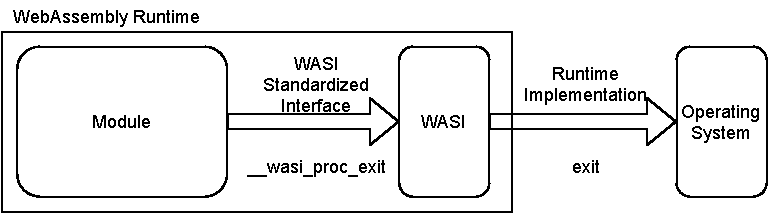
\includegraphics{Images/wasi-intro.pdf}
  \caption{A illustration of WASI}
  \label{fig:wasi-intro}
\end{figure}

\paragraph{WASI ABI Model}
WASI classifies modules into two categories, command and reactors. A command
module has a single entry function, namely \texttt{\_start} and all the other
exported functions are not accessible by the user. On the other hand, reactor
modules have an optional initialization function named \texttt{\_initialize}.
If such initialization function presents, the runtime environment is obligate
to invoke such function before calling others. The runtime environment may
invoke either the start or initializer function most once during a module's
lifetime. Additionally, every WASI-compatible model needs to export a linear
memory, named \texttt{\_memory}, and all addresses referred by modules are
offsets within such linear memory. Similarly, modules will also export an 
indirect table with the name \texttt{\_\_indirect\_function\_table}. The runtime
environment will pass function pointers through the indirect table.
Additionally, WASI requires the runtime environment to provide all WASI API
under module name \texttt{wasi\_snapshot\_preview1} 
\footnote{This will change in the future, as WASI is still in the
standardization phase.}.

\paragraph{Sandbox}
As we described above, WASI API follows WebAssembly's design philosophy, safety,
performance, portability, and compactness. WASI modules execute under a
capability-based security system to ensure the safety of the host environment.
The host runtime system will provide a sandboxed environment for each model.
For example, for filesystem access, WASI standard library C create a virtual
file system for each module with the help of libpreopen
\footnote{libpreopen: \url{https://github.com/musec/libpreopen}}
\footnote{In the more recent version of WASI libc, libpreopen is no longer
required.}.

\paragraph{Non-invasive and Extensible}
In our discussion above, one may notice that a WASI-compatible module is also a
valid WebAssembly module on its own. WASI does not introduce new instruction nor
sections to the module; instead, it provides all additional functionality
through imported external functions. The design of WASI is also highly
extensible and split into separate modules. Currently, the WASI group focuses
on developing the core part that provides most of the POSIX interface, but it
may add additional features in the future.

\section{LLVM Compiler Infrastructure}

In the last section of this chapter, we would like to have a quick overview of
the compiler pipeline design and LLVM compilation framework. Designing a robust
and efficient in terms of both generated code and compilation speed compiler is
challenging. The LLVM compile framework \cite{llvm-thesis} alleviates the
problem by introducing a standard, intermediate representation between the
compiler front end and its backend. Backend developers can target their analysis
and transformations on such IR instead of specializing in different languages.
On the other hand, frontend developers can translate the source language into
LLVM IR and expect the backend to support multiple target platforms with
efficient code generation. Figure~\ref{fig:llvm-intro} illustrates the LLVM
compilation pipeline. In this project, we are interested more in the
front of the framework. The LLVM official documentation and tutorial provide
full detail of the intermediate representation
\footnote{LLVM Language Reference Manual:
\url{https://llvm.org/docs/LangRef.html}}. Here we will only discuss several
major differences between LLVM IR and WebAssembly that help understand the
thesis. We also provide an implementation of Alder-32 hashing in LLVM IR
generated with \texttt{Clang} in figure~\ref{fig:alder-32-llvm}. 

\begin{figure}
  \centering
  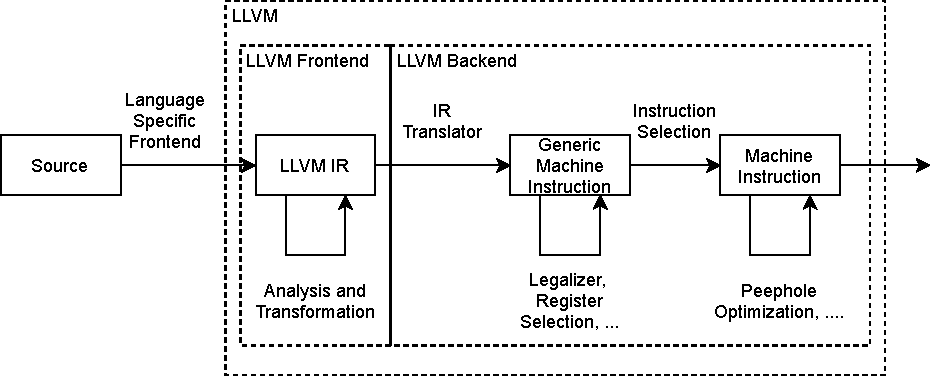
\includegraphics{Images/llvm-intro.pdf}
  \caption{A illustration of LLVM compilation pipeline}
  \label{fig:llvm-intro}
\end{figure}

\afterpage{%
\begin{figure}
  \centering
  \lstinputlisting[language=LLVM, basicstyle=\small, numbers=left]
  {Code/adler32.ll}
  \caption{Adler 32 in LLVM}
  \label{fig:alder-32-llvm}
\end{figure}
}

\paragraph{Register-based IR against Stack-based IR}
In WebAssembly, all instructions operate over an implicitly declared stack. For
example, in figure~\ref{fig:alder-32} at line $20$, a 32-bit integer constant 
instruction, \texttt{i32.const}, will push the constant value on the stack, and
a 32-bit add instruction, \texttt{i32.add} will pop two values off the stack as
left-hand-side and right-hand-side operand accordingly, then push the sum onto
the stack. On the other hand, LLVM utilizes a register-based IR, which is more
similar to what one would expect on a native machine. In 
figure~\ref{fig:alder-32-llvm}, each value for example, \texttt{\%0},
\texttt{\%1}, etc is a virtual register. In LLVM IR, there are infinite
registers. Later in the backend, the register allocation pass will map
the virtual registers into physical registers. 

\paragraph{Control Flow, Basic Block, and Phi Instruction}
As we saw in previous sections, WebAssembly has specialized instructions to
manage the program's control flow. On the other hand, LLVM took a more
traditional approach to the problem. In 1991, researchers from IBM introduced
\emph{static single assign} (SSA) form to ease writing program analysis
difficulty and transform passes \cite{ibm-ssa}. In SSA, each value has its
definition exactly once, and hence, the use-def chain is trivial to compute.
The use-def chain presents the relationship between values declarations and
used-sites in a graph. It helps the analysis pass to efficiently pinpoint the
information about values and identify if the value declaration is dead. However,
in most of the programs, values need to be able to merges from different
control-flow is required; for example, in a for-loop, the value of the loop
counter needs to change for each iteration. The SSA introduces the Phi
instructions, which marks the explicit merges of values from different execution
paths. LLVM adopts the design principle in its intermediate representation. In
figure~\ref{fig:alder-32-llvm} we have multiple phi instructions. For example,
at line $11$ and $12$, value $\%7$ and $\%8$ represent $a$ and $b$ accordingly.
We know that $a$ and $b$ initialized to $0$ and $1$ upon entry and updated in
each iteration from our C implementation. In generated LLVM IR, this merge
becomes phi instructions. For $a$ ($\%7$), if the control flow is from the
beginning of the function, we set its value to $1$, and on the other hand, if
the control flow is from the iteration, we update its value accordingly. Also,
in figure~\ref{fig:alder-32-llvm}, we have four basic blocks. A basic block
groups the maximum amount of instructions without control flow transfer. The
entry block refers to the first basic block in the function, and it is where
the control flow begins within the function body. In
figure~\ref{fig:alder-32-llvm}, this refers to basic block $\%2$. The last
instruction in the basic block is called the terminating instruction and
obligates to pass the control flow to another block, return from function or
terminate execution. Unlike WebAssembly, basic blocks can transfer control flow
to any other blocks within the same procedure except the entry block.
Additionally, phi instructions must appear before any other instructions within
the same basic block. Additionally, phi instructions must appear before any
other instructions within the same basic block, as they model the merging of
values and do not have any execution semantics. 

\paragraph{Memory and Load-Store Instruction}
The last significant difference between WebAssembly and LLVM IR is on memory
and its related instructions. As we discussed earlier, a WebAssembly module can
have access to multiple linear memories \footnote{In the current version of
WebAssembly, only one linear memory is allowed per module}. One might confuse
WebAssembly's linear memory with the concept of address space in LLVM IR. LLVM
IR associates each address with an integer value, namely address space. However,
unlike linear memory in WebAssembly, which has no difference between one and
another, the LLVM backend interprets the address space differently for various
architecture. For example, in the PTX backend, a backend target for Nvidia GPUs,
the implicit address space $0$ refers to traditional main RAM, and address space
$4$ represents the address shared by both main RAM and GPU RAM 
\footnote{An introduction for PTX backend:
\\\url{https://llvm.org/devmtg/2011-11/Holewinski_PTXBackend.pdf}}. For most of
the architecture, the implicit address space is the only address space available
to the programmer.  Another difference between WebAssembly and LLVM IR is on
load-store instruction design. Load store instructions in both languages have an
attribute on alignment. However, LLVM IR interprets this attribute differently
from WebAssembly. In WebAssembly, the alignment attribute acts as a hint to the
runtime environment. If the alignment hint is unsuitable, the runtime
environment can still execute under a possible penalty in the performance.
However, in LLVM IR, the alignment attribute is a requirement. Any memory access
that violates the alignment attribute will result in undefined behaviour,
usually a runtime panic. A load-store instruction in LLVM IR with alignment set
to one will never fail. However, it will be significantly less efficient as the
backend will likely generate byte-wise load and concatenation instructions.


We visit some of the background information that helps the understanding of the
thesis in this chapter. In the next chapter, we will start from the beginning of
the system implementation, the WebAssembly parsing and validation frontend.